\documentclass[twoside,11pt]{homework}
\usepackage{color}
\usepackage{listings}
\usepackage{graphicx} 

\coursename{Advanced Data Analysis} 

\studname{Jing Qian}    % YOUR NAME GOES HERE
\studmail{jq2282}% YOUR UNI GOES HERE
\hwNo{1}                   % THE HOMEWORK NUMBER GOES HERE
%\date{\today} % DATE GOES HERE


\begin{document}
\maketitle

\section*{Problem 1}
(a).
The sign test $S \sim Bin(25, 1/2)$. 
According to the binomial table, under $H_0$, $\alpha = P(S \ge 16) = 0.1148$.
\\\\
(b).
If $X \sim N(0.5, 1)$, $P(X \ge 0) = 0.691$.
The power of the test is the probability of rejecting the null hypothesis while the alternate is true:
%
\begin{equation}
Power = \sum\limits_{w=16}^{25}{25\choose 16} 0.691^w (1-0.691)^{25-w} = 0.782
\end{equation}
%


%%%%%%%%%%%%%%%%%%%%%
\section*{Problem 2}
(a).
$t = \frac{\overline{X}-0}{SE(\overline{X})}$ where $SE(\overline{X})$ is the standard error of $\overline{X}$.
Calculating from R,  p-value is 0.4891.
t = -0.7054, d.f. = 10 and the estimated sample mean is -0.7.

The assumption we need to make for t-test is that the samples are from a normal distribution. 
To check our assumption, we could make a QQ-plot as following:
%
%%%%%%%%%%%%%%%%%%% Fig. 1 %%%%%%%%%%%%%%%%%%%%%%%%%%%%%%
\begin{figure}[h]
\centering
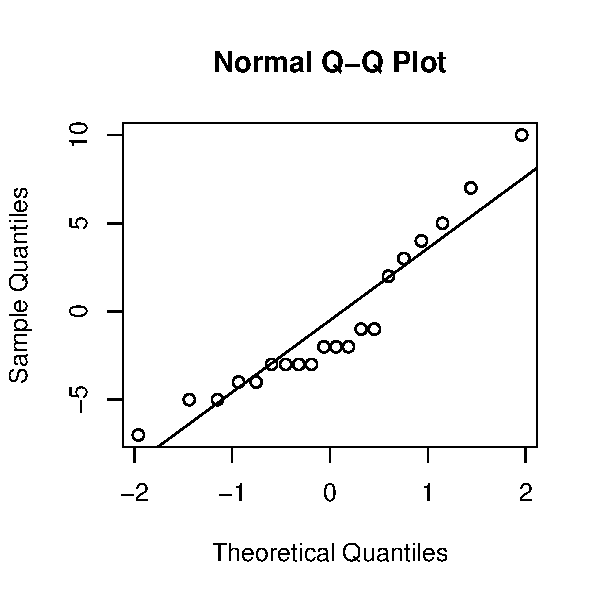
\includegraphics[scale=1]{Rplot01.pdf}
\caption{QQ plot of scores}
\label{F1}
\end{figure}
%%%%%%%%%%%%%%%%%%%%%%%%%%%%%%%%%%%%%%%%%%%%%%%%%%%%%
%
From the QQ-plot, we could see that our assumption holds.
\\\\
(b).
With t-test result from R, we could find that a 95\% confidence interval for the mean in a) is [-2.777, 1.377].
\\\\
(c).
The values of scores are: [10, -2, -1, -4,  4,  5,  3, -3, -5, -5, -2,  7, -3, -3,  2, -7, -2, -4, -1, -3].
So $S=\sum_{i=1}^{20} s(X_i - 0) = 6$.
P-value = $2\min(P(S \le 6), P(S \ge 6)) = 2 P(S \le 6)$.
Since $S \sim Bin(20, 1/2)$, we could get p-value = 0.1153, which could also be calculated by R.
\\\\
(d).
Calculate with R, the 95\% confidence interval for $\eta$ is [-3.0, 1.651].
Compared with the answer in b), we could find this CI is wider.

We could also get a rough estimate by hand:
$P(S\le 5) + P(S \ge 14) < 0.05$. 
So if $S \le 5$ or $S \ge 14$, we could reject $H_0$.
Then order scores and get data from the 6-th to 13-th, the interval is [-3, 2], which is rougher than the one calculated by R.
This one is also wider than the answer in b). 
%%%%%%%%%%%%%%%%%%%%%%%%%%%%%%
\section*{Problem 3}
(a.) \\
1. Parametric test: t-test\\
Here we could use t-test to compare the two groups.
The assumption is that data are sampled from normal distribution.
For $\sigma_1^2 \neq \sigma_2^2$, we have:
%
\begin{equation}
t = \frac{\overline{Y_1} - \overline{Y_2}}{\sqrt{\frac{s_1^2}{n_1}+\frac{s_2^2}{n_2}}}
\end{equation}
%
The distribution of $t$ could be well approximated by a t-distribution with degree of freedom equal to following:
%
\begin{equation}
d = \frac{(s_1^2/n_1 + s_2^2/n_2)^2}{(s_1^2/n_1)^2/(n_1 - 1) + (s_2^2/n_2)^2/(n_2 - 1)}
\end{equation}
%
We could calculate this values in R, having $t=-1.8481, d.f.=9.976$ and p-value = 0.09442, which is larger than $\alpha = 0.05$.
So we cannot reject $H_0$.
\\\\
2. Nonparametric test: (Wilcoxon) Mann-Whitney test\\
Here we ssume that $X$ sample and $Y$ sample are independent samples from two population which have the same shape and only differ in location.
We have:
%
\begin{equation}
W = \frac{T_X - n_1(n_1+n_2+1)/2}{\sqrt{n_1 n_2 (n_1+n_2+1)/12}}
\end{equation}
%
in which $T_X = \sum_{i=1}^{n_1}\sum_{j=1}^{n_2}I(X_i > Y_j) + \frac{n_1(n_1+1)}{2}$.
From R, we could calculate p-value = 0.1705, which is larger than $\alpha = 0.05$.
So we cannot reject $H_0$.
\\\\
(b.)\\
If we define D as a dummy variable to show whether the infant is in active-exercise group, we could fit the regression model $y=\beta_0+\beta_1 D + \epsilon$ and test $H_0: \beta_1 = 0$.

In R, we run 'model = lm(y $\sim$ D)' and 'summary(model)' to fit and get the result of fitting.
We get residual standard error: 1.484 on 10 degrees of freedom.
The calculated p-value is 0.09434, , which is larger than $\alpha = 0.05$.
So we cannot reject $H_0$.
Compared to the t-test result in a), we could find the results are quite close.

\end{document}
